%% Los cap'itulos inician con \chapter{T'itulo}, estos aparecen numerados y
%% se incluyen en el 'indice general.
%%
%% Recuerda que aqu'i ya puedes escribir acentos como: 'a, 'e, 'i, etc.
%% La letra n con tilde es: 'n.

\chapter{Métodos}
%\setcounter{section}{1}
\section{Métodos estadísticos}

\subsection{Modelo AMMI}

\textbf{Modelo AMMI clásico}

El modelo AMMI es un modelo multiplicativo en el cual se expresa la respuesta de un genotipo en un ambiente de la siguiente forma:
\begin{center}
$y_{ij}= \mu +G_i + A_j + \sum_{k=1}^q \lambda_k \alpha_{ik} \gamma_{jk}$ \vspace{1cm} $ i=1,...,g$; $ j=1,...,a$ $q=min(g-1,a-1)$
\end{center}
donde 
\begin{itemize}
\item $y_{ij}$ es el caracter fenotípico evaluado (rendimiento o cualquier otro caracter de interes) del $i$-ésimo genotipo en el $j$-ésimo ambiente,
\item $\mu$ es la media general,
\item  $G_i$ es el efecto del $i$-ésimo genotipo,
\item $A_j$ es el efecto del $j$-ésimo ambiente
\item $\sum_{k=1}^q \lambda_k \alpha_{ik} \gamma_{jk}$ es la sumatoria de componentes multiplicativas utilizadas para modelar la IGA. Siendo, $\lambda_k$ el valor singular para la  $k$-ésima PC $\alpha_{ik}$ y $\gamma_{jk}$ son los scores de las PC para el $i$-ésimo genotipo y el $j$-ésima ambiente para la $k$-ésima componente, respectivamente;
\end{itemize}

Los parámetros de IGA en el modelo AMMI se estiman por medio de la DVS de la matriz que contiene los residuos del modelo aditivo luego de ajustar por mínimos cuadrados el modelo de efectos principales.

Generalmente los dos primeros términos multiplicativos son suficientes para explicar los patrones de interacción; la variabilidad remanente se interpreta como ruido. 

Los patrones de interacción se pueden visualizar mediante los biplots GE, a menudo llamados biplots GE. El concepto del biplot fue presentado por Gabriel (1971), que consiste en una representación de las filas (individuos) y las columnas (variables) de una matriz de datos en un mismo gráfico. 

\textbf{Biplot GE}

En los modelos AMMI, el biplot GE ayuda a interpretar la variación producida por los efectos de la IGA. Se grafican en un sistema de coordenadas cartesianas de dos dimensiones los scores de los genotipos ($\alpha_{ik}$) y los ambientes ($\gamma_{jk}$), ponderados por la raíz cuadrada del autovalor correspondiente ($\lambda_k$).

Dado que los genotipos y los ambientes son definidos como vectores desde el origen (0,0) hasta sus scores, el biplot se interpreta en términos de las direcciones de vectores y sus proyecciones.\\

El módulo del vector de un ambiente da una idea de la contribución del mismo a la interacción. Los puntos de los genotipos que se encuentran próximos al origen indican que los mismos contribuyen poco a la interacción, es decir, se adaptan de igual manera a todos los ambientes. Puntos cercanos entre sí tienen patrones de interacción similares, mientras que puntos alejados entre sí tienen patrones diferentes. Cuando los marcadores (o puntos) de los ambientes y genotipos están próximos, es decir forman un aungulo $< 90^o$ ó $> 270^o$, indica que contribuyen positivamente a la interacción(hay una asociación positiva entre ese genotipo y ese ambiente); y mientras más alejados del origen se encuentre los marcadores, más fuerte será esa asociación. Una fuerte asociación positiva entre un genotipo y un ambiente se interpreta como que ese ambiente es muy favorable para ese genotipo. De manera similar, cuando los marcadores del genotipo y el ambiente están opuestos entre sí (forman un ángulo entre $90^o$ y $270^o$) se interpreta que ese ambiente es muy desfavorable para ese genotipo.\\


En la Figura \ref{fig:fig311}, se presenta un ejemplo de un biplot GE con 6 ambientes (A, B, C, D, E y F) y 10 genotipos (1, 2, 3, 4, 5, 6, 7, 8, 9 y 10). Se observa que la magnitud de los vectores de los ambientes A y E es mayor a la de los demás ambientes, es decir que esos dos ambientes son los que más contribuyen a la interacción. La cercanía de los marcadores de los genotipos 1 y 2 indica que esos genotipos tienen patrones de interacción similares, y a la vez, muy distintos a los del genotipo 4. Del biplot también se destacan las cercanías entre el genotipo 9 y el ambiente A, entre el genotipo 5 con el ambiente C, entre los genotipos 1 y 2 con el ambiente E, entre los genotipos 6, 7 y 10 con el ambiente F y entre el genotipo 4 con el ambiente D, lo que indica, debido a la gran distancia al origen, una fuerte asociación positiva entre esos genotipos y esos ambientes, es decir, esos ambientes son muy favorables para esos genotipos.\\

\begin{figure}[h]
	\begin{center}
		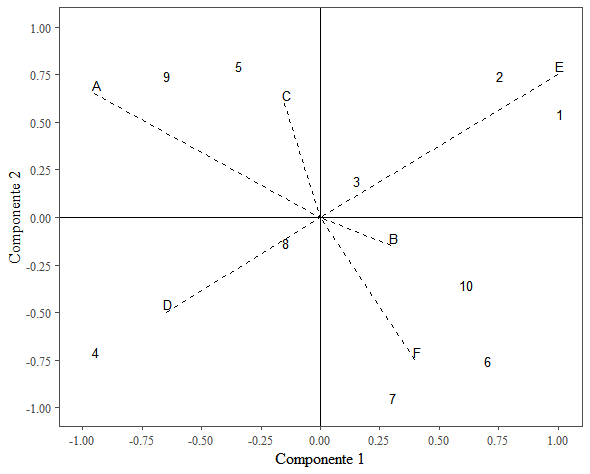
\includegraphics[width=10cm]{./Graficos/GE_biplot.png}
	\end{center}
	\caption{Ejemplo de un biplot GE}
	\label{fig:fig311}
\end{figure}

Entre las altas asociaciones negativas se puede mencionar a la del ambiente A con el genotipo 10 (marcadores opuestos en el biplot) y se interpreta que ese ambiente es considerablemente desfavorable para ese genotipo.\\

También se observa que los genotipos 3 y 8 están próximos al origen, lo que quiere decir que se adaptan en igual medida a todos los ambientes.


\textbf{Modelo AMMI robusto}

El modelo AMMI, en su forma estándar, asume que no hay valores atípicos en el conjunto de datos. La presencia de observaciones atípicas es más una regla que una excepción cuando se consideran datos agronómicos debido a errores de medición, algunas plagas / enfermedad que puede influir en algunos genotipos en un ambiente dado que resultando por ejemplo en un rendimiento inferior al esperado, o incluso debido a alguna característica inherente de los genotipos que se miden.

Rodrigues 2015 proponen una generalización robusta del modelo AMMI. La metología propuesta se puede obtener en dos etapas de la siguiente manera: primero ajustar la regresión robusta basada
en el estimador M-Huber \citep{Huber1981} para reemplazar el ANOVA; y luego utilizar un procedimiento DVS / APC robusto para reemplazar el DVS estándar. En la segunda etapa, consideraron varios métodos dando lugar a total de cinco robustos: R-AMMI, H-AMMI, G-AMMI, L-AMMI, PP-AMMI. 

El empleo de la versión robusta del modelo AMMI puede ser extremadamente útil debido a que una mala representación de genotipos y ambientes en los biplots puede dar como resultado un mala decisión con respecto a qué genotipos seleccionar para un conjunto dado de ambientes (es decir, megaambientes; \citealp{Gauch1997,Yanetal2000}). A su vez, la elección de los genotipos incorrectos pueden provocar grandes pérdidas en términos de producción de rendimiento.

Debe tenerse en cuenta que los biplots robustos mantienen las características e interpretación estándar del modelo AMMI clásico.

\subsection{Modelo SREG}

El modelo SREG (Cornelius et al., 1996; Crossa y Cornelius, 1997 y 2002) expresa el rendimiento medio de un genotipo en un ambiente en función del efecto ambiente aditivo y los efectos genotipo e interacción agrupados y en forma multiplicativa.


$y_{ij}= \mu +  A_j + \sum_{k=1}^q \lambda_k \alpha_{ik} \gamma_{jk}$ \vspace{1cm} $ i=1,...,g$; $ j=1,...,a$ $q=min(g-1,a-1)$
donde 
\begin{itemize}
\item $y_{ij}$ es la característica fenotípica evaluada (rendimiento u otra variable cuantitativa de interés) del $i$-ésimo genotipo en el $j$-ésimo ambiente,
\item $\mu$ es la media general,
\item  $G_i$ es el efecto del $i$-ésimo genotipo,
\item $A_j$ es el efecto del $j$-ésimo ambiente
\item $\sum_{k=1}^q \lambda_k \alpha_{ik} \gamma_{jk}$ es la sumatoria de componentes multiplicativas utilizadas para modelar los efectos G e IGA en forma conjunta. Siendo, $\lambda_k$ el valor singular para la  $k$-ésima IPC $\alpha_{ik}$ y $\gamma_{jk}$ son los scores de las PC para el $i$-ésimo genotipo y el $j$-ésima ambiente para la $k$-ésima componente, respectivamente;
\end{itemize}


Para visualizar conjuntamente estos dos efectos, con remoción de los efectos de ambiente (datos centrados por sitio), Yan et al. (2000) proponen los gráficos biplots GGE (Genotipe plus Genotipe-Environment). A partir de estos gráficos se puede investigar la diferenciación de mega-ambientes entre los ambientes en estudio, seleccionar cultivares superiores en un mega-ambiente dado y seleccionar los mejores ambientes de evaluación para analizar las causas de la interacción GA. Se define como mega-ambiente a un grupo de ambientes en donde los cultivares de mejor desempeño son los mismos.

\textbf{Biplot GGE}
En los modelos SREG, el biplot GGE, ayuda a interpretar conjuntamente la variación producida por los efectos principales de los G e IGA.

Para la construcción de los biplots GGE, al igual que para los biplots GE, se grafican en un sistema de coordenadas cartesianas de dos dimensiones los scores de los genotipos ($\alpha_{ik}$) y los ambientes ($\gamma_{jk}$), ponderados por la raíz cuadrada del autovalor correspondiente ($\lambda_k$).

Para una mejor comprensión de las interpretaciones que se pueden extraer del gráfico biplot GGE, se presenta un ejemplo del mismo para un ensayo de 6 ambientes (A, B, C, D, E y F) con 12 genotipos (1, 2, 3, 4, 5, 6, 7, 8, 9, 10, 11 y 12).


Para identificar los mejores genotipos en un ambiente a través del biplot GGE, Yan y Hunt (2002) sugieren trazar una recta que pase por el identificador del ambiente y el origen, la cual constituye el eje del ambiente. Luego, las proyecciones de los marcadores de los genotipos sobre ese eje, proveen un ranking de los genotipos en ese ambiente. El genotipo de mayor rendimiento en el ambiente es aquel cuya proyección sobre el eje está más alejada del origen hacia el semi-eje donde se encuentra el marcador del ambiente. Aquel cuya proyección sea la segunda más alejada del origen en ese sentido, es el de segundo mejor rendimiento y así hasta llegar al de menor rendimiento en el ambiente, que es aquel cuya proyección está más alejada del origen en sentido contrario al identificador del ambiente. La perpendicular al eje del ambiente que pasa por el origen, divide a los genotipos de rendimiento superior e inferior al promedio del ambiente.

Como se observa en la Figura \ref{fig:fig312}, el genotipo de mayor rendimiento en el ambiente D es el 4, luego le sigue el 7, luego el 8, y así sucesivamente hasta llegar al genotipo 12, que es el de peor rendimiento en ese ambiente.

\begin{figure}[h]
	\begin{center}
		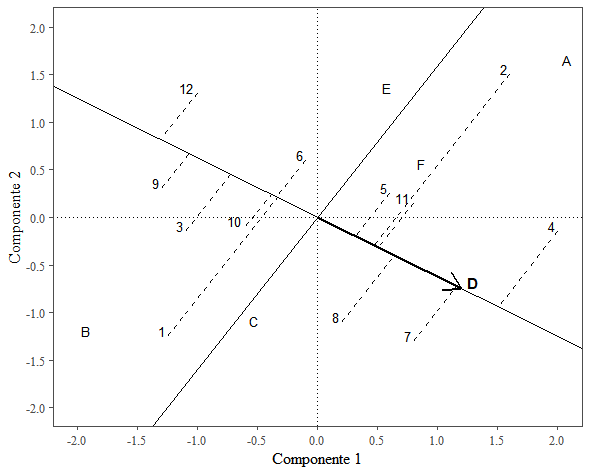
\includegraphics[width=10cm]{./Graficos/env_GGE.png}
	\end{center}
	\caption{Ranking de genotipos en el ambiente D a través del biplot GGE}
	\label{fig:fig312}
\end{figure}


Los marcadores de los genotipos 4, 7, 8, 11, 2 y 5 quedan del lado del marcador del ambiente D, de acuerdo a la división de la perpendicular que pasa por el origen, por que se interpreta que estos genotipos tienen un rendimiento mayor al promedio del ambiente D. Los restantes genotipos tienen un rendimiento inferior al promedio.


Para visualizar el desempeño de un genotipo en los diferentes ambientes, Yan y Hunt (2002) sugieren graficar una línea que una el marcador del genotipo con el origen y luego trazar otra línea perpendicular a la primera. Esta última perpendicular es la que separa los sitos favorables y desfavorables para el genotipo. Los sitios cuyos marcadores queden en el mismo lado donde está el genotipo son los mejores para ese genotipo y los restantes son aquellos donde el genotipo rinde por debajo de su promedio.



Como se puede apreciar en la Figura \ref{fig:fig313}, la perpendicular al marcador del genotipo 2, determina que los ambientes favorables para ese genotipo son A, E, F y D, en donde el mismo tiene rendimientos mayores a su promedio. Los ambientes desfavorables son B y C.
También se observa que el ambiente más favorable es el A, luego le siguen el E y el F. Si bien el ambiente D también es favorable, en ese ambiente el rendimiento del genotipo 2 es apenas superior a su rendimiento medio ya que el marcador del ambiente D, está muy cerca de la perpendicular que pasa por el origen.

\begin{figure}[h]
	\begin{center}
		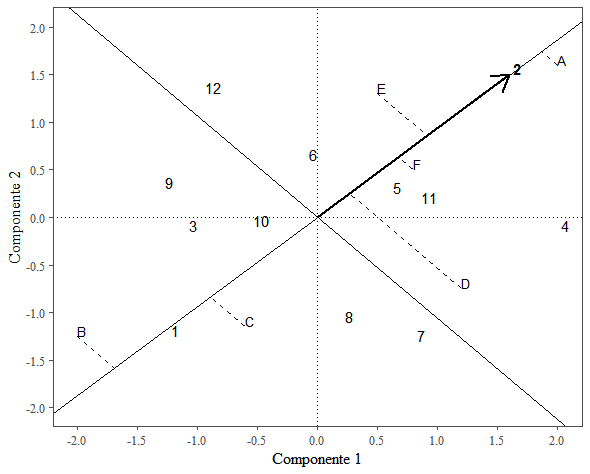
\includegraphics[width=10cm]{./Graficos/gen_GGE.png}
	\end{center}
	\caption{Ambientes favorables y desfavorables para el genotipo 2 en el biplot GGE}
	\label{fig:fig313}
\end{figure}


Para comparar dos genotipos, se propone unir mediante una línea recta los genotipos a comparar, luego trazar una línea que pase por el origen y que sea perpendicular a la línea que une a los genotipos. Esta última línea es la que separa sitios favorables a uno y a otro genotipo.


Los sitios cuyos marcadores queden en el mismo lado donde está el marcador del genotipo son los mejores para ese genotipo. Si un ambiente queda posicionado sobre la línea perpendicular, los dos genotipos tienen rendimientos similares en ese ambiente. Si dos genotipos están cercanos, sus rendimientos son similares en los ambientes evaluados. Por último, si todos los ambientes quedan a un lado de la línea perpendicular, el genotipo cuyo identificador está de ese lado rinde más que el otro en todos los ambientes.
En la Figura  \ref{fig:fig314} se puede ver la comparación de los desempeños de los genotipos 6 y 8. Los ambientes que resultan favorables para el genotipo 6 son el E, el A y el F. Mientras que los favorables para el genotipo 8 son el B, el C y el D.

\begin{figure}[h]
	\begin{center}
		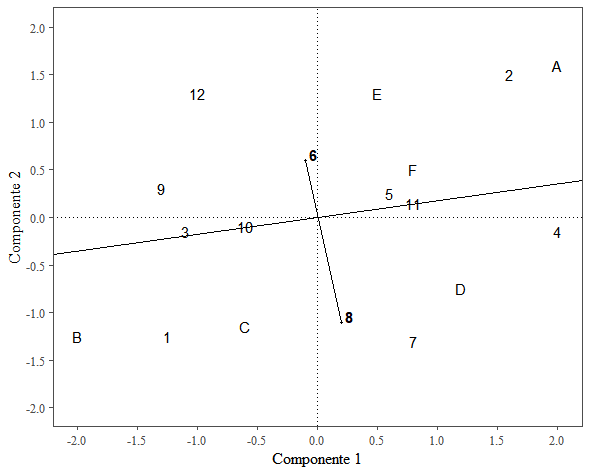
\includegraphics[width=10cm]{./Graficos/comp_gen_GGE.png}
	\end{center}
	\caption{Comparación de los genotipos 6 y 8 en el biplot GGE}
	\label{fig:fig314}
\end{figure}


Para poder identificar mega-ambientes y los mejores genotipos en cada uno de ellos se propone graficar un polígono envolvente. Este polígono se forma uniendo los genotipos más extremos en el biplot con segmentos continuados. Luego se trazan líneas rectas que pasan por el origen y que son perpendiculares a cada uno de los lados del polígono (o a sus proyecciones). De esta forma, el biplot queda dividido en cuadrantes, y los sitios que quedan dentro un mismo cuadrante se consideran pertenecientes a un mismo mega-ambiente. Generalmente cada cuadrante contiene un genotipo en el vértice, que es el de mayor rendimiento en el mega-ambiente.
En la Figura \ref{fig:fig315} se presenta el biplot GGE con el polígono envolvente y las perpendiculares a sus lados, que ayudan a la interpretación del mismo.

\begin{figure}[h]
	\begin{center}
		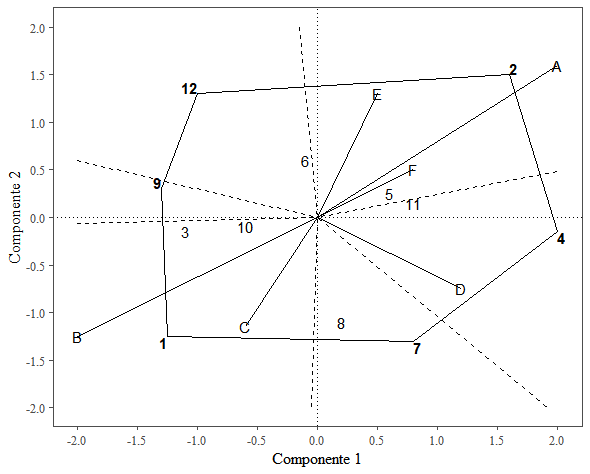
\includegraphics[width=10cm]{./Graficos/poligono_GGE.png}
	\end{center}
	\caption{Biplot GGE con el polígono envolvente y las perpendiculares a sus lados}
	\label{fig:fig315}
\end{figure}


En primer lugar se observa que los marcadores de los ambientes A y B son mayores a los restantes, lo que indica que la variabilidad en esos ambientes es superior, es decir, en ellos es donde mejor se diferencian los efectos de los genotipos.
Las perpendiculares a los lados del polígono envolvente determinan tres mega-ambientes:
\begin{itemize}
\item uno formado por los ambientes A, E y F, en donde el genotipo de mejor desempeño es el 2 (se
encuentra en el vértice del polígono encerrado por las perpendiculares).
\item otro está formado solo por el ambiente D y el genotipo ganador en él es el 4, y
\item  el tercer mega-ambiente lo componen los ambientes B y C, en este caso el genotipo ganador es el 1.
\end{itemize}

Si se identifican distintos mega-ambientes, la selección de genotipos debe hacerse para cada mega-ambiente en particular. Los genotipos se seleccionan en base a su desempeño y a su estabilidad a través de los ambientes.
En el biplot, se puede definir un eje medio para todos los ambientes pertenecientes a un mismo mega-ambiente. Para ello se calcula la media de scores promediando los scores de la componente 1 y la componente 2 de los ambientes pertenecientes al mega-ambiente. Una vez obtenidos estos promedios, se traza una línea recta entre ese punto medio y el origen, que se denomina eje de la media de scores de ambientes. A continuación se traza una línea que pase por el origen y que sea perpendicular a la línea
media de scores de ambientes. Estas dos líneas constituyen ``el eje de coordenadas de ambiente medio''.
Las proyecciones de los marcadores de los genotipos sobre el eje de la media de scores de ambientes da un ranking de los rendimientos de los genotipos en ese mega-ambiente. A su vez la magnitud de la proyección de los marcadores de los genotipos a la perpendicular al eje de ambientes da una idea de la estabilidad. Cuanto mayor sea esta magnitud, más inestable será el genotipo.
En este ejemplo se calcula el ambiente medio para un mega-ambiente, en la Figura 4.6 se presenta el gráfico del eje medio para el mega-ambiente formado por los ambientes A, E y F. El promedio de los scores de la primer componentes es 1,00 y el de la segunda es 1,133, por lo que el punto medio que determina la dirección del eje es (1; 1,133), que está graficado con un círculo en la Figura \ref{fig:fig316}.

\begin{figure}[h]
	\begin{center}
		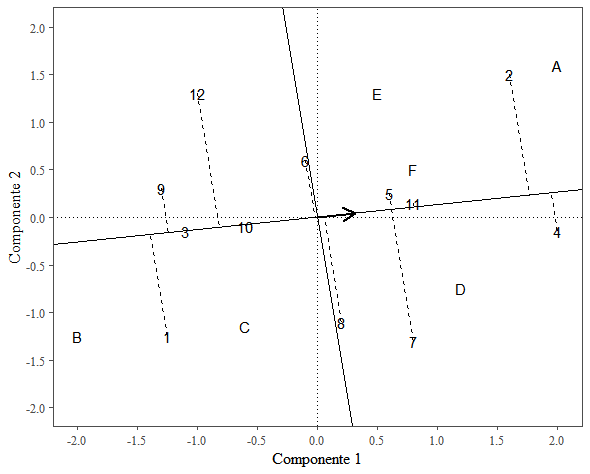
\includegraphics[width=10cm]{./Graficos/mean_stab_GGE.png}
	\end{center}
	\caption{Eje de coordenadas de ambiente medio para un mega-ambiente en el biplot GGE}
	\label{fig:fig316}
\end{figure}

Como se puede observar en el biplot el orden de los genotipos (de mayor a menor rendimiento) es: 2, 4, 12, 11, 5, 6 todos ellos con rendimientos superiores al promedio, seguidos por los de rendimiento menor al promedio: el 10, 9, 7, 3 y por último el 1, el de peor rendimiento medio en ese mega-ambiente.
Debido a que las proyecciones sobre el eje perpendicular al eje medio de ambiente dan una idea de la estabilidad, se observa que el genotipo 12, el 9, el 7 y el 4 son los más inestables. También se observa que el genotipo 2, además de tener el mejor rendimiento medio es de los más estables en el megaambiente.


\subsection{Métodos de imputación}


Una limitación importante que presentan los modelos multiplicativos (AMMI y SREG) es que requieren que el conjunto de datos este completo, es decir no admiten valores perdidos. Aunque los EMA están diseñados para que todos los genotipos se evalúen en todos los ambientes, la presencia de valores faltantes es muy común, debido por ejemplo a la incorporación de nuevos genotipos, errores de medición o causas naturales como la destrucción de plantas por animales, inundaciones o durante la cosecha.

Entre las posibles soluciones para tratar un conjunto de datos con observaciones perdidas: el uso de un subconjunto completo de datos, eliminando aquellos genotipos que tienen valores faltantes (Ceccarelli et al., 2007, Yan et al., 2011), completar datos faltantes con la media ambiental, o imputación de los valores faltantes mediante estimaciones utilizando, por ejemplo, un modelo multiplicativo (Kumar et al., 2012).

Se han propuesto numerosas metodologías para superar el problema de valores ausentes en el conjunto de datos, entre las cuales se encuentran:

\begin{itemize}
\item EM-AMMI: Gauch y Zobel (1990) desarrollaron este enfoque mediante el cual se imputa utilizando el algoritmo de maximización de la esperanza (EM, del inglés \emph{Expectation-Maximization}) incorporando el modelo AMMI. Consiste en un procedimiento iterativo que funciona de la siguiente forma: .............
Dependiendo del número de términos multiplicativos empleados, el método de imputación puede denominarse EM-AMMI0, EM-AMMI1, etc. (Gauch y Zobel 1990). Los estudios de Caliński y col. (1992), Piepho (1995), Arciniegas-Alarcón y Dias (2009) y Paderewski y
Rodrigues (2014) mostraron que se obtienen los mejores resultados para la imputación con modelos AMMI al incluir como máximo una componente multiplicativa.
\end{itemize}
\begin{itemize}
\item EM-SVD: Perry (2009a) propone un método de imputación que combina el algoritmo EM con DVS. Este método reemplaza los valores faltantes de una matriz $G \times E$ inicialmente por valores arbitrarios para obtener una matriz completa, y luego la DVS se calcula iterativamente en esa matriz. Al final del proceso, cuando las iteraciones alcanzan estabilidad, se obtiene la matriz imputada.
.....Podria ponerlo tambien de manera formal... pero creo que con esto basta
\end{itemize}
\begin{itemize}
\item EM-PCA:
\end{itemize}
\begin{itemize}
\item Gabriel Eigen: Arciniegas-Alarcón et al. (2010) propuso un método de imputación que combina regresión y aproximación de rango inferior usando DVS. El método reemplaza inicialmente las celdas faltantes por valores arbitrarios, y posteriormente el
las imputaciones se refinan a través de un esquema iterativo que define una partición de la matriz para cada valor que falta a su vez y utiliza una regresión lineal de columnas (o filas) para obtener el nueva imputación. En esta regresión, la matriz de diseño se aproxima por una matriz de menor rango usando la DVS.
\end{itemize}
\begin{itemize}
\item WGabriel Eigen:
\end{itemize}

Vale la pena señalar que el modelo de análisis no siempre será el mismo que el modelo de imputación.





\section{Paquete de R}

%https://oscarperpinan.github.io/R/Paquetes.html 
Una librería o paquete (\emph{package}) es una colección de objetos creados y organizados siguiendo un protocolo fijo que garantiza la ausencia de errores (de sintaxis) en la programación. Éstos son las unidades fundamentales de un código reproducible de R ya que incluyen funciones reutilizables, la documentación que describe cómo usar cada una de ellas y, además datos de ejemplo. 

Los pasos necesarios para la creación de un paquete son:
\begin{itemize}
\item Creación del esqueleto del paquete.
\item Inclusión de los objetos que contendrá el paquete (funciones y/o datos).
\item Redacción de la documentación.
\item Redacción de la viñeta.
\item Compilación del paquete en Linux y creación de la versión para Windows.
\item Instalación.
\item Prueba y publicación.
\end{itemize}


Para la cración del paquete se utilizan numerosas funciones incluidas en el paquete \emph{devtools} en el cual se encuentran un conjunto de paquetes que admiten varios aspectos del desarrollo de paquetes. Por lo tanto, antes de comenzar a crear el paquete se deben instalar el mismo como se indica a continuación:\\

\begin{lstlisting}
# Instalar el paquete devtools desde CRAN
install.packages("devtools")

# Instalar el paquete devtools desde GitHub:
devtools::install_github("r-lib/devtools")
\end{lstlisting}

\subsection{Esqueleto y estructura del paquete}

Para crear la estructura del paquete se utiliza la función create\_package(). El principal y único argumento requerido por dicha función es el directorio donde el nuevo paquete se alojará. Por lo general, si el directorio se llama ``geneticae'', entonces el nombre del paquete también será ``geneticae'':


\begin{lstlisting}
# Cargar la libreria devtools
library(devtools)

# Crear el paquete geneticae
create_package("C:/Users/Julia/Desktop/geneticae")
\end{lstlisting}


El resultado de ejecutar la función create\_package() es un paquete con los siguientes componentes:
\begin{itemize}
\item Un directorio R/.
\end{itemize}
\begin{itemize}
\item DESCRIPTION, un archivo simple cuyo objetivo es almacenar metadatos importantes sobre el paquete, epecifica el título, la versión del mismo, identifica al autor y brinda un mail de contacto, una breve descripción del paquete, la lista de los paquetes que el paquete creado necesita para funcionar, la licencia, entre otros.

El contenido básico en un archivo DESCRIPTION es:
\end{itemize}

\begin{verbatim}
Package: geneticae
Title: What the Package Does (One Line, Title Case)
Version: 0.0.0.9000
Authors@R: 
    person(given = "First",
           family = "Last",
           role = c("aut", "cre"),
           email = "first.last@example.com",
           comment = c(ORCID = "YOUR-ORCID-ID"))
Description: What the package does (one paragraph).
License: What license it uses
Encoding: UTF-8
LazyData: true
\end{verbatim}




\begin{itemize}
\item Un archivo NAMESPACE
\end{itemize}

También puede incluir un archivo de proyecto de RStudio pkgname.Rproj, que hace que su paquete sea fácil de usar con RStudio; .Rbuildignore enumera los archivos que se necesitan, pero que no deben incluirse al compilar el paquete R desde la fuente; .gitignore anticipa el uso de Git e ignora algunos archivos estándar detrás de escena creados por R y RStudio.

\subsection{Creación de funciones y conjuntos de datos}

Una vez creada la estructura del paquete se debe comenzar a incluir las funciones que contendrá. Cada una de ellas debe ser guardada en un archivo de extensión .R, en el subdirectorio R/. La funcion use\_r() crea y/o abre un script de la carpeta R/.

Una vez creada una función, para probarla se utiliza load\_all() que simula el proceso de construcción, instalación y conexión del paquete. Permite que las funciones creadas estén disponible rápidamente para uso interactivo, del mismo modo que si se hubiera construido e instalado el paquete y luego cargado a través de library(geneticae).

Muy frecuentemente se utilizan funciones de otros paquetes, para ello se utiliza la función use\_package() que agrega el paquete  a lista de los paquetes que el paquete creado necesita para funcionar del archivo DESCRIPTION.

A menudo es útil incluir datos en un paquete, con estos se proporcionan casos de uso convincentes para las funciones del paquete. La ubicación más común para los datos es data/, siendo cada archivo de este directorio un .RData que sólo contiene un  objeto. Para esto, se utiliza la funció usethis::use\_data(). Se puede observar que el archivo DESCRIPTION creado con la función create\_package() contiene el campo LazyData: true, lo cual genera que los conjuntos de datos no ocuparán ninguna memoria hasta que los use.

\subsection{Documentación}

La documentación es uno de los aspectos más importantes del código, sin ella, los usuarios no sabrán cómo usar el paquete. Existen múltiples formas de documentar un paquete, la forma estándar es escribir archivos .Rd en la carpeta man, los cuales utilizan una sintaxis personalizada, basada en LaTeX. Sin embargo, el paquete \emph{roxygen2}, utilizado en este trabajo, convierte los comentarios con formato especial en archivos .Rd. Esta última proporciona una serie de ventajas sobre la estándar:

\begin{itemize}
\item El código y la documentación son adyacentes, de modo que cuando el código se modifique, será fácil actualizar la documentación.

\item Inspecciona dinámicamente los objetos que está documentando, para que pueda agregar automáticamente los datos que de otra forma se deben escribir a mano.

\item Resume las diferencias en la documentación de los métodos S3 y S4, los genéricos y las clases, por lo que necesita aprender menos detalles.
\end{itemize}

Además de generar archivos .Rd, \emph{roxygen2} también creará el archivo NAMESPACE.

El flujo de trabajo para crear la documentación con el paquete \emph{roxygen2} es el siguiente:
\begin{itemize}
\item Agregar comentarios a los archivos .R, los cuales comienzan con \#' y preceden a una función. La primera oración se convierte en el título y el segundo párrafo es una descripción de la función. Seguidamente, las funciones son documentadas, la mayoría de las funciones tienen tres etiquetas: @param, @examples y @return.

\begin{itemize}
\item  @param describe los parámetros de la función, indica de que clase es el parámetro y para que sirve.
\item @examples proporciona un código ejecutable que muestra cómo usar la función en la práctica. 
\item @return describe el resultado de la función. 
\end{itemize}
\end{itemize}
\begin{itemize}

\item Ejecutar devtools::document() para convertir los comentarios de roxygen en archivos .Rd. 

\end{itemize}

Roxigen permite utilizar la descripción de los parámetros de otras funciones usando @inheritParams source function. Esta etiqueta traerá toda la documentación de los parámetros que no están documentados en la función actual, pero que están documentados en la función fuente. La fuente puede ser una función en el paquete actual, vía @inheritParams function, u otro paquete, vía @inheritParams package::function.

A diferencia de las funciones que son documentadas directamente, para los objetos en data/, se debe crear un archivo y guardarlo en el directorio R/.



\subsection{Viñetas}

EXPLICAR UN POCO QUE ES UNA VINETA


Para crear la viñeta, se utiliza usethis::use\_vignette(``my-vignette''). La misma crea un directorio vignettes/, agrega las dependencias necesarias a DESCRIPTION y redacta la viñeta. Las tres componentes fundamentales de la misma son las siguientes:

\begin{itemize}
\item El bloque inicial de metadatos, que contiene la siguiente información:
\end{itemize}

\begin{verbatim}
---
title: "Vignette Title"
output: rmarkdown::html_vignette
vignette: >
  %\VignetteIndexEntry{Vignette Title}
  %\VignetteEngine{knitr::rmarkdown}
  \usepackage[utf8]{inputenc}
---
\end{verbatim}

\begin{itemize}
\item Markdown para formatear texto.
\item Knitr para interpretar texto, código y resultados.
\end{itemize}

\subsection{Pruebas del flujo de trabajo}

Las pruebas resultan fundamentales en el desarrollo de paquetes, asegura que el código haga lo que realmente se desea. Existen pruebas informales como aquellas realizadas con la función load\_all. Sin embargo, estas pruebas interactivas pueden convertirse en scripts reproducibles, los cuales resultan superiores debido a que:

\begin{itemize}
\item Se indica explícitamente cómo debería comportarse el código, provocando que los errores solucionados no vuelvan a ocurrir.

\item El código que es fácil de probar generalmente está mejor diseñado, reduce la duplicación en el código. Como resultado, las funciones serán más fáciles de probar, comprender y trabajar.

\item Si toda la funcionalidad del paquete tiene una prueba asociada, se pueden hacer grandes cambios sin preocuparse por generar errores.
\end{itemize}


Para probar el flujo de trabajo se utiliza la función usethis::usetestthat(). Esta crea un directorio tests/testthat, agrega testthat al campo Suggests en el archivo DESCRIPTION y además, crea un archivo tests/testthat.R que ejecuta todas las pruebas cuando R CMD check se ejecuta. 

Las pruebas se organizan jerárquicamente: las expectativas se agrupan en pruebas que se organizan en archivos :
\begin{itemize}
\item Una expectativa describe el resultado esperado de un cálculo.

\item Una prueba agrupa múltiples expectativas para probar la salida de una función simple, un rango de posibilidades para un solo parámetro de una función más complicada o una funcionalidad estrechamente relacionada de varias funciones.

\item Un archivo agrupa múltiples pruebas relacionadas. Los archivos reciben un nombre legible para humanos con context().
\end{itemize}

Se utiliza la funcion test(), para ejecutar todas las pruebas creadas a la vez. Las pruebas también se ejecutan cada vez que se utiliza la función check() descripta a continuación. 

\subsection{Compilación e instalación}

Mediante la función load\_all se fue simulando el proceso de construcción, instalación y conexión del paquete, con el fin de ir probando las funciones creadas. Sin embargo, R CMD check ejecutado en el shell o check(), es el estándar de oro para verificar que un paquete R esté en pleno funcionamiento. La misma verificará que no haya errores de sintaxis o no se generen warnings. Está compuesto por más de 50 chequeos individuales entre los cuales se encuentran: la estructura del paquete, el archivo descripción, namespace, el código de R, los datos, la documentación, entre otros. Se aconseja realizar verificaciones completas de que todo funciona a medida que se van incorporando funciones ya que si se incorporan muchas y luego se verifican será dificil identificar y resolver los problemas. Una vez que las verificaciones completas no encuentran errores, advertencias o notas, se ejecuta la función install(), con el objetivo de instalar el paquete en la biblioteca.


\subsection{Publicación}
%https://rsanchezs.gitbooks.io/ciencia-de-datos-con-r/paquetes/paquetes.html
Un repositorio es el lugar dónde están alojados los paquetes y desde el cuál se pueden descargarlos. Entre los repositorios más populares de paquetes R se encuentran:

\begin{itemize}
\item \textbf{CRAN}: es el principal repositorio de paquetes de R, está coordinado por la fundación R. Previa a la publicación en este repositorio el paquete debe pasar por diferentes pruebas para asegurar que cumple con las políticas de CRAN.

\item \textbf{Bioconductor}: se trata de un repositorio específico para bioinformática. Del mismo modo que CRAN, tiene sus propias políticas de publicaciones y procesos de revisión.

\item \textbf{GitHub}: a pesar que no es específico para R, github es con toda seguridad el repositorio más popular para la publicación de proyectos \emph{open source} (del inglés, código abierto). Su popularidad procede del espacio ilimitado que proporciona para el alojamiento de proyectos \emph{open source}, la integración con git (un software de control de versiones) y, la facilidad de compartir y colaborar con otras personas. Una de sus desventajas es que no proporciona procesos de control.

\item \textbf{R-Forge} y \textbf{RForge}: son entornos de desarrollo de paquetes y repositorios. Eso significa que incluyen control de fuente, seguimiento de errores y otras características. Puede obtener versiones de desarrollo de paquetes de estos.
\end{itemize}

El paquete \emph{geneticae} se encuentra en GitHub, para instalar el mismo se deben seguir las siguientes instrucciones:\\


\begin{lstlisting}
library(devtools)
install_github("jangelini/geneticae") 
\end{lstlisting}





{\Huge{(Ideas de: https://mastering-shiny.org/dependency-tracking.html)}}

\section{Shiny APP}
Una aplicación web es una aplicación o herramienta informática accesible desde cualquier navegador, bien sea a través de internet (lo habitual) o bien a través de una red local. 
Estas aplicaciones son muy populares hoy en día para los usuarios no expertos, debido a la facilidad de su uso, ya que no requiere de una instalación en el ordenador del usuario, simplemente se accede a través de un navegador. Por lo que es posible utilizar una aplicación web desde desde cualquier dispositivo con conexión a internet, ya sea un ordenador, un smartphone o una tablet, es decir que es independiente del sistema operativo del usuario. Otra gran ventaja es el bajo consumo de recursos, ya que la mayor parte del tiempo estos se consumen en el servidor donde se encuentra alojada la aplicación, que generalmente tiene mucha más potencia de cómputo que cualquier ordenador personal.

%https://datanalytics.com/libro_r/shiny.html
Shiny es un paquete R que te permite crear aplicaciones web interactivas, permitiendo exhibir un trabajo de R a través de un navegador web para que cualquiera pueda usarlo. 

Crear aplicaciones web puede resultar difícil para la mayoría de los usuarios de R debido a que se necesita un conocimiento profundo de las tecnologías web como HTML, CSS y JavaScript; y además hacer aplicaciones interactivas complejas requiere un análisis cuidadoso de los flujos de interacción para asegurarse de que cuando una entrada cambie, solo se actualicen las salidas relacionadas. Sin embargo, shiny hace que sea mucho más fácil para el programador R crear aplicaciones web al proporcionar un conjunto de funciones de interfaz de usuario (UI para abreviar) que generan el HTML, CSS y JavaScript que necesita para tareas comunes. Esto significa que no se necesita conocer los detalles de HTML / CSS / JS.

Shiny fomenta la separación del código que genera tu interfaz de usuario (el \emph{front-end}) del código que impulsa el comportamiento de tu aplicación (el \emph{backend}. Por lo tanto, Los dos componentes clave de cada una Shiny APP son: 

\begin{itemize}
\item ui (\emph{user interfaz}): la interfaz de usuario controla el diseño de la aplicación, recibe los inputs y
muestra los outputs en el navegador.
\item server, funciones de R que contienen las instrucciones que se necesitan para construir los resultados de los análisis incluidos en la aplicación.
\item shinyApp, función que crea objetos de aplicación Shiny a partir de ui / servidor.
\end{itemize}

El esquema interno de la aplicación puede observarse en la Figura \ref{fig:fig321}. 

\begin{figure}[h]
\begin{center}
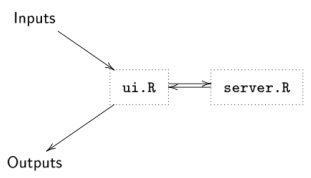
\includegraphics[width=7cm]{./Graficos/figura7}
\end{center}
\caption{Esquema interno de la aplicación.}
\label{fig:fig321}
\end{figure}


La programación reactiva es un estilo de programación que enfatiza valores que cambian con el tiempo, y cálculos y acciones que dependen de esos valores. Esto es importante para las aplicaciones Shiny porque son interactivas: los usuarios cambian los controles de entrada (arrastrando controles deslizantes, escribiendo en cuadros de texto y marcando casillas de verificación), lo que hace que la lógica se ejecute en el servidor (leer CSV, subconjunto de datos y modelos de ajuste) que finalmente resultan en actualización de salidas (parcelas de respuesta, actualización de tablas).

Para que las aplicaciones Shiny sean útiles, necesitamos dos cosas:

Las expresiones y las salidas deben actualizarse siempre que cambie uno de sus valores de entrada. Esto asegura que la entrada y la salida permanezcan sincronizadas.

Las expresiones y las salidas deben actualizarse solo cuando una de sus entradas cambia. Esto garantiza que las aplicaciones respondan rápidamente a la entrada del usuario, haciendo la cantidad mínima.

Es relativamente fácil satisfacer una de las dos condiciones, pero es mucho más difícil satisfacer ambas. Para ver por qué y para ver cómo podríamos atacar el problema básico con otros estilos de programación, utilizaremos un ejemplo muy simple, eliminando la complejidad adicional de una aplicación web y enfocándonos en el código subyacente.


\subsection{Flujo de trabajo}

El esta sección se motrará como mejorar dos flujos de trabajo de Shiny importantes: El ciclo de desarrollo básico de crear aplicaciones, realizar cambios y experimentar con los resultados; y la Depuración, el arte y el oficio de descubrir qué salió mal con su código y las soluciones de lluvia de ideas para solucionarlo.\\


\textbf{1.\hspace{1cm} Flujo de trabajo de desarrollo}\\


El objetivo de optimizar el flujo de trabajo de desarrollo es reducir el tiempo entre hacer un cambio y ver el resultado. Cuanto más rápido se pueda iterar, más rápido se podrá experimentar y más rápido podrá obtener su Shiny. Aquí hay dos flujos de trabajo principales para optimizar: crear la aplicación por primera vez y acelerar el ciclo iterativo de ajustar el código y probar los resultados.


\textbf{Creación de la Shiny APP}


Para poder crear una shiny APP se debe tener instado R, RStudio ya que tiene algunas características agradables específicamente para autoría, depuración y desplegando aplicaciones estas aplicaciones, y lo siguientes paquetes:

\begin{lstlisting}
install.packages(c(
  "ggforce", "shiny", "shinythemes", "tidyverse", "vroom" 
))
\end{lstlisting}

Para crear una Shiny APP, lo más simple es crear un nuevo directorio para su aplicación y crear un sólo archivo llamado app.R en él. Este archivo se usará para indicarle a Shiny cómo debería verse la aplicación y cómo debería comportarse.

\begin{lstlisting}[frame=single]
library(shiny)
ui<- ...
server<- ...
shinyApp(ui = ui, server = server)
\end{lstlisting}


Por lo tanto, en el archivo app.R se realizan las siguientes tareas:

\begin{itemize}
\item Carga el paquete shiny: 
\begin{lstlisting} 
library(shiny) 
\end{lstlisting}
\item Define la interfaz de usuario, la página web HTML con la que los usuarios interactúan.
\item Especifica el comportamiento de nuestra aplicación definiendo la  función server. 
\item Se ejecuta shinyApp(ui, server)para construir e iniciar una aplicación Shiny desde la interfaz de usuario y el servidor.
\end{itemize}


La sesión de R estará monitoreando la aplicación y ejecutando las reacciones de la aplicación mientras la aplicación Shiny esté activa, por lo que no podrá ejecutar ningún comando.

En todo tipo de programación, es una mala práctica tener código duplicado; puede ser un desperdicio computacional y, lo que es más importante, aumenta la dificultad de mantener o depurar el código.

En la secuencia de comandos R tradicional, utilizamos dos técnicas para lidiar con el código duplicado: capturamos el valor usando una variable o capturamos el cálculo con una función. Desafortunadamente, ninguno de estos enfoques funciona aquí y se necesita un nuevo mecanismo: expresiones reactivas . Una expresión reactiva tiene una diferencia importante con una variable: sólo se ejecuta la primera vez que se llama y luego almacena en caché el resultado de la misma hasta que necesite actualizarse.


\textbf{Ver los cambios}


Al crear o modificar la aplicacion, se la ejecuta para poder ver los cambios realizados, por lo que el dominio de flujo de trabajo de desarrollo es especialmente importante. La primera forma de reducir la velocidad de iteración es evitar hacer clic en el botón "Ejecutar aplicación" y, en su lugar, aprender el método abreviado de teclado Cmd/Ctrl+ Shift+ Enter. Esto le brinda el siguiente flujo de trabajo de desarrollo:

\begin{enumerate}
\item Escribe un código.
\item Inicie la aplicación con Cmd/Ctrl+ Shift+ Enter.
\item Experimentar interactivamente con la aplicación.
\item Cierra la aplicación.
\item Ir a 1.
\end{enumerate}


Otra forma de reducir aún más la velocidad de iteración es activar la recarga automática (options(shiny.autoreload = TRUE)) y luego ejecutar la aplicación en un trabajo en segundo plano, como se describe en https://github.com/sol-eng/background-jobs/tree/master/shiny-trabajo. Con este flujo de trabajo tan pronto como guarde un archivo, su aplicación se reiniciará: no es necesario cerrarla y reiniciarla. Esto conduce a un flujo de trabajo aún más rápido:
\begin{enumerate}
\item Escriba un código y presione Cmd/Ctrl+ Spara guardar en el archivo.
\item Experimentar interactivamente.
\item Ir a 1.
\end{enumerate}
La principal desventaja de esta técnica es que debido a que la aplicación se ejecuta en un proceso separado, es considerablemente más difícil de depurar.

De manera predeterminada, cuando ejecuta la aplicación, aparecerá en una ventana emergente. Sin embargo ,existen otras dos opciones que puede elegir del menú desplegable \emph{Run App}
\begin{enumerate}
\item La ejecución en el panel del visor es útil para aplicaciones más pequeñas porque puede verla al mismo tiempo que ejecuta el código de la aplicación.
\item Ejecutar en un navegador externo es útil para aplicaciones más grandes, o si desea verificar que su aplicación se ve exactamente de la manera que espera en el contexto que la mayoría de los usuarios la verán.
\end{enumerate}


\textbf{2.\hspace{1cm} Depuración}\\


Entre los problemas que pueden surgir al crear una Shiny app se encuentran los siguientes:

\begin{itemize}
\item Error inesperado. Este es el caso más fácil, porque obtendrá un rastreo que le permitirá averiguar exactamente de dónde proviene el error. Una vez que haya identificado el problema, deberá probar sistemáticamente su suposición hasta que encuentre una diferencia entre sus expectativas y lo que realmente está sucediendo. El depurador interactivo es una herramienta poderosa para este proceso.
\item No obtiene ningún error, pero un valor es incorrecto. Aquí, generalmente es mejor transformar esto en el primer problema utilizando stop()para arrojar un error cuando se produce el valor incorrecto.
\item Todos los valores son correctos, pero no se actualizan cuando espera. Este es el problema más desafiante porque es exclusivo de Shiny, por lo que no puede aprovechar sus habilidades de depuración de R.

\end{itemize}


Una vez localizado la fuente del error, la herramienta más poderosa es el depurador interactivo. El depurador detiene la ejecución y le brinda una consola R interactiva donde puede ejecutar cualquier código para descubrir qué salió mal. Hay dos formas de iniciar el depurador:

\begin{itemize}
\item Agregar una llamada a la función browser() en código fuente. Esta es la forma estándar de R de iniciar el depurador interactivo, y funcionará sin embargo, se está ejecutando brillante.
\item Agregar un punto de interrupción RStudio haciendo clic a la izquierda del número de línea. Puede eliminar el punto de interrupción haciendo clic en el círculo rojo. La ventaja de los puntos de interrupción es que no son código, por lo que nunca tendrá que preocuparse por registrarlos accidentalmente en su sistema de control de versiones.
\end{itemize}





\subsection{Compartiendo una Shiny Web App}

Una vez creada la aplicación, resulta conveniente ponerlas a disposición de los usuarios. En este caso la Shiny Web App encuentra disponible en el servidor de CONICET \url{www.cefobi.com}. Además el proyecto se encuentra en GitHub \url{https://github.com/jangelini/shinyAPP_geneticae}. 
